\begin{figure}[ht]
    \centering
    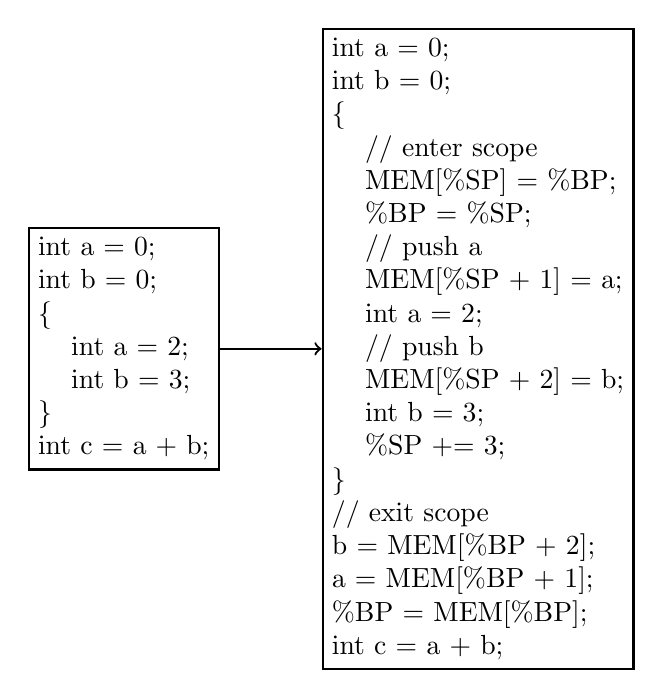
\begin{tikzpicture}[node distance={45mm}, thick, main/.style = {draw}] 
        \node[main, align=left] (Orig) {
            \code{int a = 0;}\\
            \code{int b = 0;}\\
            \code{\{}\\
            \code{\hspace{12pt}int a = 2;}\\
            \code{\hspace{12pt}int b = 3;}\\
            \code{\}}\\
            \code{int c = a + b;}
        };
        \node[main, align=left] (Scoped) [right of=Orig] {
            \code{int a = 0;}\\
            \code{int b = 0;}\\
            \code{\{}\\
            \comment{\hspace{12pt}// enter scope }\\
            \red{\code{\hspace{12pt}MEM[\%SP] = \%BP;}}\\
            \red{\code{\hspace{12pt}\%BP = \%SP;}}\\
            \comment{\hspace{12pt}// push a }\\
            \red{\code{\hspace{12pt}MEM[\%SP + 1] = a;}}\\
            \code{\hspace{12pt}int a = 2;}\\
            \comment{\hspace{12pt}// push b }\\
            \red{\code{\hspace{12pt}MEM[\%SP + 2] = b;}}\\
            \code{\hspace{12pt}int b = 3;}\\
            \red{\code{\hspace{12pt}\%SP += 3;}}\\
            \code{\}}\\
            \comment{// exit scope }\\
            \red{\code{b = MEM[\%BP + 2];}}\\
            \red{\code{a = MEM[\%BP + 1];}}\\
            \red{\code{\%BP = MEM[\%BP];}}\\
            \code{int c = a + b;}
        };
        \draw[->] (Orig) -- (Scoped);
    \end{tikzpicture} 
    \caption{A scope handling example for \CoBBl, where \code{MEM} represents the write-once memory used for stack simulation. Note that this transformation takes place only if \code{a} and \code{b} are selected by \CoBBl's register spilling.}
    \label{fig:continuation-passing}
\end{figure}